%%% LaTeX Template: Article/Thesis/etc. with colored headings and special fonts
%%%
%%% Source: http://www.howtotex.com/
%%% Feel free to distribute this template, but please keep to referal to http://www.howtotex.com/ here.
%%% February 2011
%%%
%%% Modified January 2018 by CDM

%%%  Preamble
\documentclass[11pt,letterpaper]{article}
\usepackage[margin=1.0in]{geometry}
\usepackage[T1]{fontenc}
\usepackage[bitstream-charter]{mathdesign}
\usepackage[latin1]{inputenc}					
\usepackage{amsmath}						
\usepackage{xcolor}
\usepackage{cite}
\usepackage{hyphenat}
\usepackage{graphicx}
\usepackage{float}
\usepackage{subfigure}
\usepackage{sectsty}
\usepackage[compact]{titlesec} 
\usepackage[tablegrid]{vhistory}
\allsectionsfont{\color{accentcolor}\scshape\selectfont}

%%% Definitions
\definecolor{accentcolor}{rgb}{0.0,0.0,0.5} 
\newcommand{\teamname}{Runtime Terrors}
\newcommand{\productname}{Turing Board}
\newcommand{\coursename}{CSE 4316: Senior Design I}
\newcommand{\semester}{Fall 2021}
\newcommand{\docname}{System Requirements Specification}
\newcommand{\department}{Department of Computer Science \& Engineering}
\newcommand{\university}{The University of Texas at Arlington}
\newcommand{\authors}{Sahaj Amatya \\ Sarker Nadir Afridi Azmi \\ Kendall Buchanan \\ Keaton Koehler \\ Happy Ndikumana \\ Lydia Sarver}

%%% Headers and footers
\usepackage{fancyhdr}
	\pagestyle{fancy}						% Enabling the custom headers/footers
\usepackage{lastpage}	
	% Header (empty)
	\lhead{}
	\chead{}
	\rhead{}
	% Footer
	\lfoot{\footnotesize \teamname \ - \semester}
	\cfoot{}
	\rfoot{\footnotesize page \thepage\ of \pageref{LastPage}}	% "Page 1 of 2"
	\renewcommand{\headrulewidth}{0.0pt}
	\renewcommand{\footrulewidth}{0.4pt}

%%% Change the abstract environment
\usepackage[runin]{abstract}			% runin option for a run-in title
%\setlength\absleftindent{30pt}			% left margin
%\setlength\absrightindent{30pt}		% right margin
\abslabeldelim{\quad}	
\setlength{\abstitleskip}{-10pt}
\renewcommand{\abstractname}{}
\renewcommand{\abstracttextfont}{\color{accentcolor} \small \slshape}	% slanted text

%%% Start of the document
\begin{document}

%%% Cover sheet
{\centering \huge \color{accentcolor} \sc \textbf{\department \\ \university} \par}
\vspace{1 in}
{\centering \huge \color{accentcolor} \sc \textbf{\docname \\ \coursename \\ \semester} \par}
\vspace{0.5 in}
\begin{figure}[h!]
	\centering
   	
\includegraphics[width=0.40\textwidth]{images/turing_logo.png}
\end{figure}
\vspace{0.5 in}
{\centering \huge \color{accentcolor} \sc \textbf{\teamname \\ \productname} \par}
\vspace{0.5 in}
{\centering \large \sc \textbf{\authors} \par}
\newpage


%\vspace{1 in}
%\centerline{January 13th, 2012}
%\newpage

%%% Revision History
\begin{versionhistory}
  	\vhEntry{0.1}{10.22.2021}{SA}{document creation}
  	\vhEntry{0.2}{10.28.2021}{SA}{completed sections 1 and 2}
  	\vhEntry{0.3}{11.04.2021}{KB|LS}{Proofread Draft}
\end{versionhistory}
\newpage

%%% Table of contents
\setcounter{tocdepth}{3}
\tableofcontents
\newpage

%%% List of figures and tables (optional)
\listoffigures
%\listoftables
\newpage

\section{Product Concept}
This section provides a high-level statement of your product concept - what it is intended to do and how it is intended to be used. Include in this header paragraph, a brief synopsis of what is described here. For example, this header paragraph might say something like: "This section describes the purpose, use and intended user audience for the X product. X is a system that performs Y. Users of X will be able to Z..."

\subsection{Purpose and Use}
This is where you describe in a brief, yet clear and concise, manner what your product should do and how you expect it should be used.

\subsection{Intended Audience}
This is where you describe the intended audience(s) of your product. If this product were to be made available publicly or commercially, who would purchase or use it? Is the product designed for a particular customer, or an overall class of customers? Is it intended for general use, or is it a specific component of a more complex system?

\begin{figure}[h!]
	\centering
   	
\includegraphics[width=0.60\textwidth]{images/test_image}
    \caption{X conceptual drawing}
\end{figure}

\newpage
\section{Product Description}
This section provides the reader with an overview of the Turing Board. The primary operational aspects of the the Turing Board, from the perspective of end users, are defined here. The key features and functions found in the Turing Board, as well as critical user interactions and user interfaces are described in detail.

\subsection{Features \& Functions}
When desired, the Turing Board will follow the user side by side at a walking pace. When called upon, it will summon itself to the user's location from a parked spot. However, users will not be able to take advantage of the autonomous features when they mount the board. The change in inertia spawned by a computer generated movement of the longboard puts the user at great risk of losing balance when taking off, braking, and especially turning. This changes the balance of the system as a whole. Such a problem is not an issue in household autonomous vehicles such as a self-driving car because the change in inertia only affects the balance of the user and not the car in any significant way. 

The feature set of the Turing Board also consists of the collection and display of ride analytics.

Visually, the Turing Board is anticipated to share the form of any regular electric skateboard, with the only difference being that it is going to have a camera mounted on the nose end. The parts will consist of a deck, underneath the deck will comprise of an encasing that will house the battery, computation module, turning mechanism hardware, trucks and motorized wheels. The placement of the camera module is anticipated to be on the top of the board. 

On the software side, the items include native Android and iOS apps to interface with the Turing Board.

\subsection{External Inputs \& Outputs}
GPS information is a critical entity that will be involved in both external input and output scenarios. We will need the account for the GPS information of both the user and the board. The user authentication is handled by the Google Firebase Authentication API paired with the Google Firebase Cloud Firestore API acting as a cloud database. 

\subsection{Product Interfaces}
Here are some of the screenshots of what the application interface will look like for the end-user. 
\begin{figure}
    \centering
    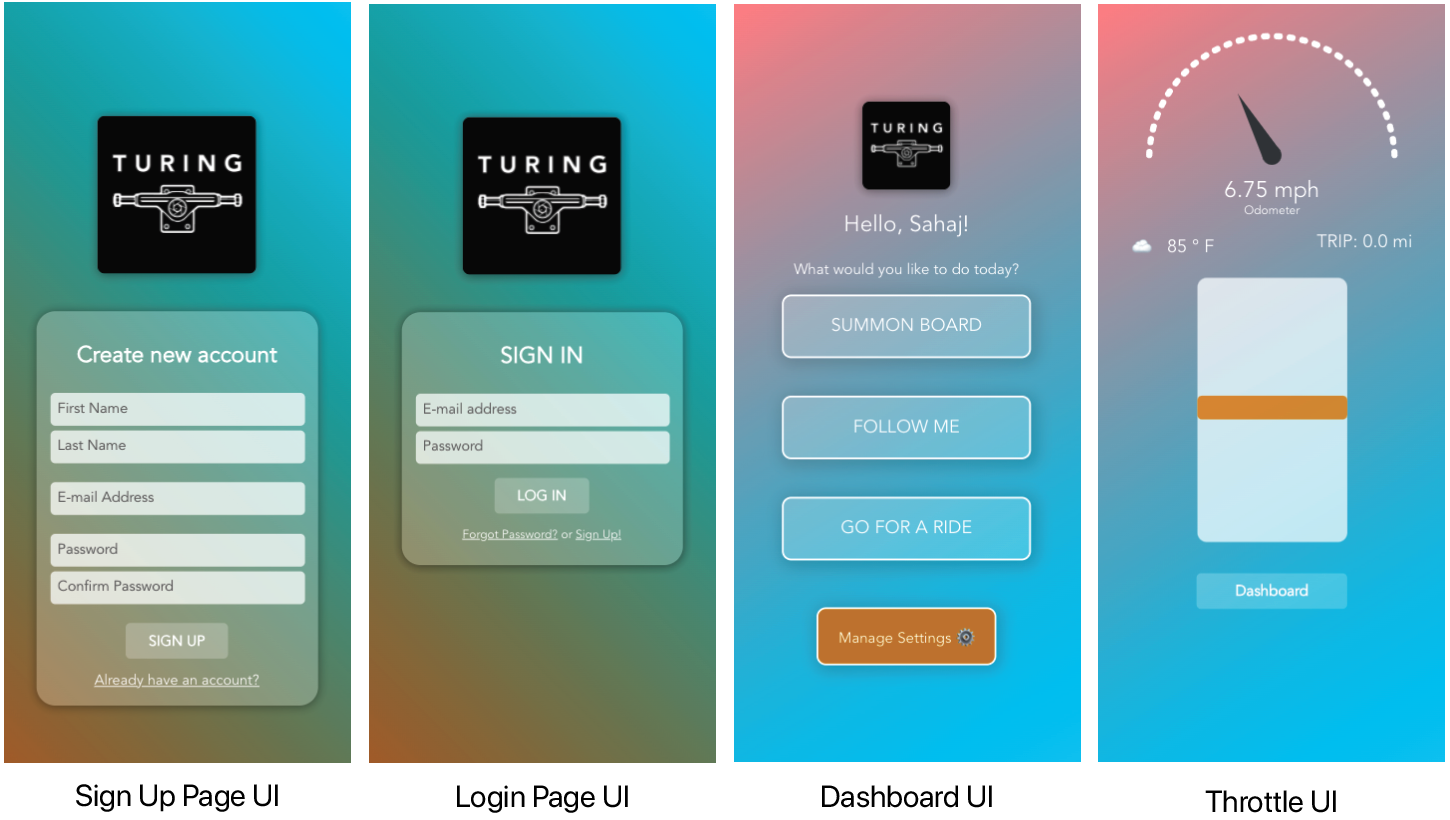
\includegraphics[width=0.9\textwidth]{images/UI.png} % first figure itself
    \caption{User Interface Screenshots}
\end{figure}

%Specify what all operational (visible) interfaces look like to your end-user, administrator, maintainer, etc.Show sample/mocked-up screen shots, graphics of buttons, panels, etc.  Refer to the critical externalinputs and outputs described in the paragraph above.
\newpage
\section{Customer Requirements}
Include a header paragraph specific to your product here. Customer requirements are those required features and functions specified for and by the intended audience for this product. This section establishes, clearly and concisely, the "look and feel" of the product, what each potential end-user should expect the product do and/or not do. Each requirement specified in this section is associated with a specific customer need that will be satisfied. In general Customer Requirements are the directly observable features and functions of the product that will be encountered by its users. Requirements specified in this section are created with, and must not be changed without, specific agreement of the intended customer/user/sponsor.

\subsection{GPS}
\subsubsection{Description}
As part of the autonomous navigation system, the GPS would provide coordinate data which would allow the program to know the position of the longboard which would be used to draw vectors to aid with navigation to a target coordinate.
\subsubsection{Source}
The GPS built into the phone will be used to get the current location of the longboard.
\subsubsection{Constraints}
The GPS coordinates provided by the phone should be precise without jumping from one value to another too much.
\subsubsection{Standards}
Conforms to the standard Global Positioning System.
\subsubsection{Priority}
High

\subsection{Remote}
\subsubsection{Description}
Instead of having a separate remote, a free-to-download app will be made available which can be used to summon the board, enable the follow-me feature, and control the speed of the wheels. The app currently uses React as the framework of choice for the front-end and is hosted publicly on Netlify. It uses sockets for communication, but a better approach we found is Bluetooth which would make the process of data transfer very simple and easy. The app  will soon be changed to using React Native to support both Android and IOS. The reason for this is to ensure full compatibility without having to worry about browser versions.
\subsubsection{Source}
Native Android and IOS application making use of Bluetooth to communicate with the longboard.
\subsubsection{Constraints}
Since the rider of the longboard will be going quite fast, the transmission of data needs to be reduced as much as possible. Latency should be minimized.
\subsubsection{Standards}
Bluetooth 4.0/5.0 for maximum compatibility.
\subsubsection{Priority}
High

\newpage
\section{Packaging Requirements}
The product will be shipped pre-assembled which would include the turning mechanism, camera, and Jetson already screwed onto a standard longboard. The only thing not plugged in would be the batteries which the user has to connect themselves. The firmware for the product will come pre-installed where the user would only be required to pair the device with the mobile app to make use of it. An ankle bracelet with ArUco Tags for the follow me feature and a power supply for charging the batteries would also be included as part of the purchase.

% \subsection{Requirement Name}
% \subsubsection{Description}
% Due to the nature of the product, the main point of failure is the turning mechanism which needs to be protected using bubble wrap with zip ties holding it in place to prevent it from shaking during shipping. Anything electrical which might not be inside of an enclosure will be contained inside of ant-static bags to prevent static from killing the parts. The Ankle bracelet will be packaged separately in a hard casing to prevent it from bending or being compressed during shipping. The batteries would come packaged inside of an insulated bag alongside the power supply. All the components would be placed inside of the delivery box which would have dedicated sections for each part.
% \subsubsection{Source}
% These are some of the locations from which the parts are being sourced:\\
% 1. Adafruit\\
% 2. Amazon\\
% 3. eBay
% \subsubsection{Constraints}
% One of the major constraints is to make sure that the board does not move around too much whilst shipping as it contains sensitive components which might get chipped off in a scenario where a screw comes loose, and the PCB hits the inside of the casing. Also, the shipping environment should have a fairly constant temperature as electrical components are heavily affected by temperature which might cause the parts to degrade. The latter scenario is an extreme case.
% \subsubsection{Standards}
% The shipment should be handled with care and not thrown around which moving from one shipment container to another.
% \subsubsection{Priority}
% High

\subsection{Board Design (Look \& Feel)}
\subsubsection{Description}
The look and feel is incredibly important for a final product. It is the polish that makes the shoe shine, after all. The finished longboard topside will have a minimalist look similar to a normal longboard or eboard, custom protective housings for all electrical components on the underside, and Turing Board custom grip tape signed by all team members.
\subsubsection{Source}
Runtime Terrors
\subsubsection{Constraints}
The electronics mounted to the underside must be thin enough to avoid scraping or bottoming out on bumpy sidewalks.
\subsubsection{Standards}
The underside will be where all electrical components are mounted, with holes drilled and milled accordingly for each mounting screw. The topside will, preferably, be flush with no screws/nuts sticking out or epoxy left un-sanded. All components will have widths short enough to fit within the constraints of the board dimensions leaving no overhanging objects. Grip tape will be applied after all drilling, milling, and sanding has been done to leave a clean topside.
\subsubsection{Priority}
Medium

\subsection{Frontend}
\subsubsection{Description}
The Turing Board's remote will be controlled via a phone app available on iOS and Android. The app was built using React Native. The backend is being handled by Google's Firebase API.
\subsubsection{Source}
Runtime Terrors
\subsubsection{Constraints}
N/A
\subsubsection{Standards}
N/A
\subsubsection{Priority}
Critical

\subsection{Dampeners}
\subsubsection{Description}
Excessive vibrations within the electronic housing can cause destructive resonance and render the board non-functional. In order to absorb these vibrations foam dampeners will be installed around all essential parts of the internal components.
\subsubsection{Source}
This requirement comes from the hardware engineers responsible for designing the internal components.
\subsubsection{Constraints}
Foam that is rigid enough to absorb vibrations caused by fast movement over uneven terrain but will not compress enough to cause damage to the internals.
\subsubsection{Standards}
No standards will be used.
\subsubsection{Priority}
High

\newpage
\section{Performance Requirements}
This section highlights an overview of the Turing Board's performance. At its heart, the Turing board should be able to follow a target user and it should be able to be summoned from a parking location. The board should be able to use computer vision, the turning mechanism and the propulsion mechanism to navigate. The board should also be able to function as a normal electric long-board when a user is on it. Throughout this section, each major performance requirement will be examined in detail, including its constraints, standards and priority.

\subsection{Turning Angle}
\subsubsection{Description}
For our autonomous turning mechanism, the front wheels will only be able to turn with an angle of \±30$^{\circ}$ from the neutral position (0$^{\circ}$ A.K.A. facing forward).
\subsubsection{Source}
Kendall Buchanan (Runtime Terrors)
\subsubsection{Constraints}
The turning angle should be constrained to \±30$^{\circ}$ to allow the board decent turning angles while not overextending and causing the board to topple over.
\subsubsection{Standards}
Based on research conducted when determining a maximum possible turning angle, the standard car has a turning angle of \±30$^{\circ}$ and this sounded like a good standard to build off of.
\subsubsection{Priority}
High

\subsection{Limited Slip Differential}
\subsubsection{Description}
One feature we are looking to possibly include is a limited slip differential (LSD) to help with turning smoothly and efficiently in autonomous mode.
\subsubsection{Source}
Happy Ndikumana (Runtime Terrors)
\subsubsection{Constraints}
Since the trucks of a longboard are designed as a single piece (mostly) with an embedded axle, we would only be able to implement this LSD on the rear, motor-driven wheels. Also, how the rear wheels are constructed makes a physical LSD impossible. Therefore we would code in an electronic LSD into the motor controls.
\subsubsection{Standards}
As stated above, the physical construction of the longboard trucks, front and rear, make it impossible to implement a physical LSD. An electronic LSD would simply use the motor controller to simulate an LSD by making the inner wheel spin slower (or the outer wheel spin faster) when turning, thus making turning smoother and sharper.
\subsubsection{Priority}
Low

\subsection{Battery}
\subsubsection{Description}
A 288Wh, 8000mAh, 36 V battery will provide power to the entire system. For the preliminary design, the voltage will be stepped down using a Buck Converter providing ~19V to the Jetson TX2. There will be an open 5V and 3.3V terminal if there is a need to connect external power to sensors and microcontrollers.
\subsubsection{Source}
Specified by the team member (Sarker Nadir Afridi Azmi)
\subsubsection{Constraints}
The power used by the entire system should be minimized to ensure the the longboard can operate for at least an hour or two with a rider before it needs to be charged.
\subsubsection{Standards}
288Wh, 8000mAh, 36 V
\subsubsection{Priority}
High
\newpage
\section{Safety Requirements}
The Turing Board is a scientific achievement combining the power of electricity, the ingenuity of longboarding, and the innovation of autonomous machine learning. This, however, also comes with a slew of safety concerns and features to be followed closely. The longboard must be kept in a dry place of a nominal temperature. Do not use around heavy machinery or vehicles. Do not use in the vicinity of sheer drops or falls. Do not use around children. Must be age 18+ to use. A helmet MUST BE WORN AT ALL TIMES. Recommended only for use by experienced boarders. 

\subsection{Laboratory equipment lockout/tagout (LOTO) procedures}
\subsubsection{Description}
Any fabrication equipment provided used in the development of the project shall be used in accordance with OSHA standard LOTO procedures. Locks and tags are installed on all equipment items that present use hazards, and ONLY the course instructor or designated teaching assistants may remove a lock. All locks will be immediately replaced once the equipment is no longer in use.
\subsubsection{Source}
CSE Senior Design laboratory policy
\subsubsection{Constraints}
Equipment usage, due to lock removal policies, will be limited to availability of the course instructor and designed teaching assistants.
\subsubsection{Standards}
Occupational Safety and Health Standards 1910.147 - The control of hazardous energy (lockout/tagout).
\subsubsection{Priority}
Critical

\subsection{National Electric Code (NEC) wiring compliance}
\subsubsection{Description}
Any electrical wiring must be completed in compliance with all requirements specified in the National Electric Code. This includes wire runs, insulation, grounding, enclosures, over-current protection, and all other specifications.
\subsubsection{Source}
CSE Senior Design laboratory policy
\subsubsection{Constraints}
High voltage power sources, as defined in NFPA 70, will be avoided as much as possible in order to minimize potential hazards.
\subsubsection{Standards}
NFPA 70
\subsubsection{Priority}
Critical

\subsection{RIA robotic manipulator safety standards}
\subsubsection{Description}
Robotic manipulators, if used, will either housed in a compliant lockout cell with all required safety interlocks, or certified as a "collaborative" unit from the manufacturer.
\subsubsection{Source}
CSE Senior Design laboratory policy
\subsubsection{Constraints}
Collaborative robotic manipulators will be preferred over non-collaborative units in order to minimize potential hazards. Sourcing and use of any required safety interlock mechanisms will be the responsibility of the engineering team.
\subsubsection{Standards}
ANSI/RIA R15.06-2012 American National Standard for Industrial Robots and Robot Systems, RIA TR15.606-2016 Collaborative Robots
\subsubsection{Priority}
Critical

\subsection{Weather Proof Casing}
\subsubsection{Description}
A water-proof case is needed to protect the sensitive electronic components of the Turing board from environmental conditions. In addition to keeping out moisture the case will act as a barrier from any debris that could cause damage while the board is at high speeds (rocks, sticks, etc).
\subsubsection{Source}
This requirement is from the hardware engineers.
\subsubsection{Constraints}
The profile of the container must be slim enough to not touch the ground while the board is turning. The case must be strong enough to withstand limited physical stress. A rubber gasket or seal is necessary to prevent liquid from touching the sensitive equipment.
\subsubsection{Standards}
No standards were used.
\subsubsection{Priority}
High

\subsection{Alarm or Buzzer for Improper Use}
\subsubsection{Description}
The Turing Board's autonomous capabilities are not intended for use with a rider on the long board. A weight sensor will trigger a buzzer to sound if the user attempts to ride while under autonomous operations or if a change in weight is detected while the turning mechanism is engaged.
\subsubsection{Source}
This requirement is from both the hardware and software engineers.
\subsubsection{Constraints}
The buzzer will need to be loud enough to catch the attention of the user despite environmental distractions.
\subsubsection{Standards}
No standards were used.
\subsubsection{Priority}
Low

\subsection{Board Response to Accidents}
\subsubsection{Description}
The Turing Board's response to an accident is necessary. In the regretful case a user should fall off the board, the board must take the appropriate measures to make the user's life easier and keep bystanders safe. There are two main response expected if a user falls off the board. If the user falls of the board and the Turing Board is still in the user's vicinity, then the moment the sensor reading changes from "user weight" to "no weight", the Turing Board stops. This same mechanism applies in the case the user falls off and lands far away from the board. In these events, the board should autonomously find its way back to the user.
\subsubsection{Source}
These responses were specified by the group.
\subsubsection{Constraints}
The board must have a reliable weight sensor that will always return the right weight. A faulty reading could cause an accident itself by suddenly stopping the board.
\subsubsection{Standards}
If the Turing board is within 3 meters of the user after the user falls off, the board will automatically stop.\hfill \break
If the Turing board is outside of a 3 meters parameter of the user after an accident and emergency stop, the board must autonomously roll back to its user. 
\subsubsection{Priority}
Low

\subsection{Mode Switch}
\subsubsection{Description}
The role of the mode switch is to disengage autonomous mode. With the help of the weight sensor, it will be determined if a user, a small load or nothing is on top of the board. When a user is on the Turing board, we must prioritize their safety. The way we will do this is by disengaging autonomous mode and making sure the turning mechanism is locked at 0 degrees. This will ensure the Turing board can be operated as a normal electric long-board and prevent any accidents that could be caused by a misaligned front truck. 
\subsubsection{Source}
The role and mechanics of the mode switch were specified by the team.
\subsubsection{Constraints}
When a set weight is exceeded, meaning a user is on the board, autonomous mode will be disengaged and the turning mechanism will be rotated and locked at 0 degrees for the user's safety.
\subsubsection{Standards}
If a weight greater than 23 kg (50 lbs) is detected, the "mode switch" will be triggered. It will disengage autonomous mode, rotate the trucks back to 0 degrees and the trucks will be locked at that position using solenoids.
\subsubsection{Priority}
Critical
\newpage
\section{Maintenance \& Support Requirements}
The Turing Board is ultimately meant to be a full product sent to a customer ready to ride basically out of the box. For this reason, the majority of the maintenance and support items are abstracted from the user's view. We will provide a user manual to the user, but other than that it would largely be up to the supporting team to resolve any technical issue with the board. For the app, we are hosting our login admin portal on Google's Firebase Authentication. 

\subsection{Firebase Authentication Admin Portal}
\subsubsection{Description}
The Turing Board's authentication is hosted through Google's Firebase. It currently uses the free Spark Plan. Through this portal, an admin would have the ability to manage users, reset passwords, and monitor authentication usage. 
\subsubsection{Source}
Sahaj Amatya \& firebase.google.com/pricing
\subsubsection{Constraints}
The Spark Free plan for Firebase only allows for 10,000 authentications per month.
\subsubsection{Standards}
N/A
\subsubsection{Priority}
Moderate

\newpage
\section{Other Requirements}
The Turing Board has important features that don't quite fit into the other requirements section criteria, leaving it for the other requirements section. These have just as important an impact on the product as other requirements. These are generally the more innovative requirements to implement special features. As our project progresses and grows, these requirements may grow as well, allowing new features to be added.

\subsection{Follow Along}
\subsubsection{Description}
An identifiable marker worn on the rider (around the ankle or back of a shoe) will be recognized and tracked by the CV on the longboard to allow it to follow along with the wearer as they walk or run. The CV will be able to track if the marker is to the left or the right of the camera center and also measure the distance to the marker to help it keep pace with the wearer.
\subsubsection{Source}
Sahaj Amatya
\subsubsection{Constraints}
Camera is only able to track/recognize up to 20ft. Low-light conditions or partially obscured markers will have trouble being recognized.
\subsubsection{Standards}
Must be easily tracked in multiple lighting conditions (mainly daytime conditions) and at multiple angles.
\subsubsection{Priority}
High

\newpage
\section{Future Items}
In this last section, you will reiterate all requirements that are listed as priority 5. This is repetitive, but necessary as a concise statement of features/functions that were considered/discussed and documented herein, but will NOT be addressed in the prototype version of the product due to constraints of budget, time, skills, technology, feasibility analysis, etc. Use the following format for this section.

\subsection{Requirement Name}
\subsubsection{Description}
Detailed requirement description...
\subsubsection{Source}
Source
\subsubsection{Constraints}
Detailed description of applicable constraints...
\subsubsection{Standards}
List of applicable standards
\subsubsection{Priority}
Priority
\newpage

%%% References
\bibliographystyle{plain}
\bibliographystyle{reference/IEEEtran_custom}
\bibliography{reference/refs}{}

\end{document}